\chapter{Approximate Bayesian methods}\label{chap15}

\section*{Solutions of Exercises}\label{sec11_1}
\begin{enumerate}[leftmargin=*]

\item \textbf{g-and-k distribution for financial returns continues I}

Simulate a dataset following the specification given in the g-and-k distribution for financial returns example. Set $\theta_1 = 0.8$, $a = 1$, $b = 0.5$, $g = -1$, and $k = 1$, with a sample size of 500, and use the same priors as in that example. Implement the ABC accept/reject algorithm from scratch using one million prior draws, selecting the 1,000 draws with the smallest distance.\footnote{Note that this setting does not satisfy the asymptotic requirements for Bayesian consistency. However, it serves as a pedagogical exercise.}

\begin{itemize}
	\item Perform a linear regression adjustment using the posterior draws of our ABC-AR algorithm (ABC-AR-Adj).
	\item Compare the results with those obtained using the ABC-AR implementation in the \textit{EasyABC} package, ensuring that the computational time is relatively similar between both implementations.
	\item Compare the posterior results of ABC-AR, ABC-AR-Adj and EasyABC with the population values.
\end{itemize}

\textbf{Answer:}

The following code implements our ABC-AR algorithm, following the steps outlined in the ABC-AR Algorithm of the book. Users can observe that a linear regression adjustment is applied; however, due to multicollinearity issues, one summary statistic is omitted in the prediction step (see the \textit{abc} package for alternative regression adjustments).  

Figure \ref{figABCown} presents the posterior distributions of $\theta_1$, $g$, and $k$ using both our ABC implementations and the \textit{EasyABC} package. We observe that our algorithms provide less information about $\theta_1$ compared to the \textit{EasyABC} implementation. Conversely, our algorithms offer more information about $g$ and $k$ than the \textit{EasyABC} function. Additionally, regression adjustment helps center the posterior distributions of $g$ and $k$ around the population parameters. But, this is no the case regarding $\theta_1$. Moreover, applying regression adjustment introduces a degree of smoothness to the distributions. Overall, in all implementations, the 95\% credible intervals encompass the population values.

\begin{figure}[!h]
	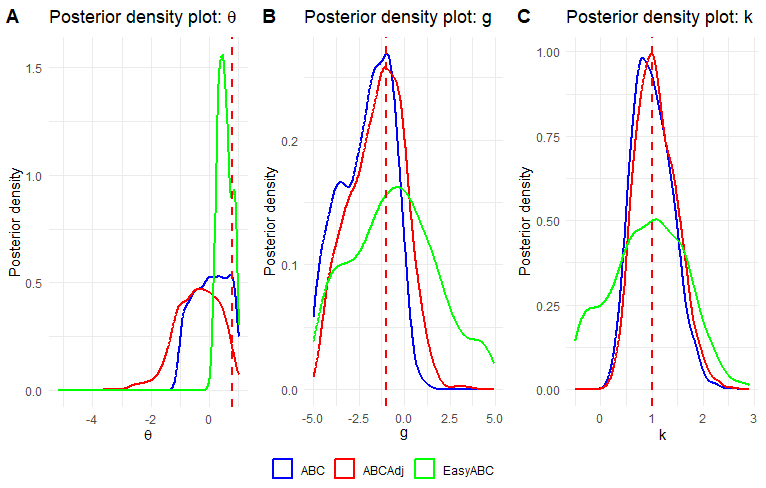
\includegraphics[width=340pt, height=200pt]{Chapters/chapter15/figures/ABCown.png}
	\caption[List of figure caption goes here]{Posterior distributions using approximate Bayesian computation accept/reject: g-and-k distribution.}\label{figABCown}
\end{figure}

\begin{tcolorbox}[enhanced,width=4.67in,center upper,
	fontupper=\large\bfseries,drop shadow southwest,sharp corners]
	\textit{R code. Approximate Bayesian computation accept/reject algorithm: g-and-k distribution simulation}
	\begin{VF}
		\begin{lstlisting}[language=R]
rm(list = ls()); set.seed(010101)
# Simulate g-and-k data
RGKnew <- function(par) {
	z <- NULL
	theta <- par[1]; a <- par[2]; b <- par[3]; g <- par[4]; k <- par[5]
	e <- rnorm(n + 1)
	for(t in 2:(n + 1)){
		zt <- e[t] + theta * e[t-1]
		z <- c(z, zt)
	}
	zs <- z / (1 + theta^2)^0.5
	x <- a + b * (1 + 0.8 * (1 - exp(-g * zs)) / (1 + exp(-g * zs))) * (1 + zs^2)^k * zs
	return(x)
}
# Summary statistics
SumSt <- function(y) {
	Oct <- quantile(y, c(0.125, 0.25, 0.375, 0.5, 0.625, 0.75, 0.875))
	eta1 <- Oct[6] - Oct[2]
	eta2 <- (Oct[6] + Oct[2] - 2 * Oct[4]) / eta1
	eta3 <- (Oct[7] - Oct[5] + Oct[3] - Oct[1]) / eta1
	autocor <- acf(y, lag = 2, plot = FALSE)
	autocor[["acf"]][2:3]
	Etay <- c(Oct, eta1, eta2, eta3, autocor[["acf"]][2:3])
	return(Etay)
}
# Population parameters
theta1 <- 0.8; a <- 1; b <- 0.5; g <- -1; k <- 1
parpop <- c(theta1, a, b, g, k)
n <- 500
y <- RGKnew(par = parpop) 
##### ABC Function#####
ABC <- function(S, a, y) {
	prior <- cbind(runif(S,-1,1), runif(S,0,5), runif(S,0,5), runif(S,-5,5), runif(S,-0.5,5))
	Z <- apply(prior, 1, RGKnew)
	EtasZ <- apply(Z, 2, SumSt)
	Etay <- SumSt(y) 
	Dist <- sapply(1:S, function(l) {
		dist(rbind(Etay, EtasZ[, l]))
	})
	OrdPrior <- prior[order(Dist), ]
	SelPrior <- OrdPrior[1:round(S * a), ]
	SelSumSt <- t(EtasZ)[1:round(S * a), ]
	return(list(SelPrior = SelPrior, SelSumSt = SelSumSt))
}
S <- 1000000
a <- 0.001
tick <- Sys.time()
ResABC <- ABC(S = S, a = 0.001, y = y)
tock <- Sys.time()
tock - tick
PostABC_ARown <- ResABC[["SelPrior"]]
\end{lstlisting}
	\end{VF}
\end{tcolorbox}

\begin{tcolorbox}[enhanced,width=4.67in,center upper,
	fontupper=\large\bfseries,drop shadow southwest,sharp corners]
	\textit{R code. Approximate Bayesian computation accept/reject algorithm: g-and-k distribution simulation}
	\begin{VF}
		\begin{lstlisting}[language=R]
# Regression adjusted ABC
X <- ResABC[["SelSumSt"]]-matrix(SumSt(y), S*a, 12, byrow = TRUE)
PostABC_ARownRegAd <- PostABC_ARown
for(j in 1:5){
	Reg <- lm(PostABC_ARown[,j] ~ X)
	# Coefficient of regressor 9 is na.
	PostABC_ARownRegAd[,j] <- PostABC_ARown[,j] - X[,-9]%*%Reg$coefficients[-c(1,9)]
}
RGKnewSum <- function(par) {
	z <- NULL
	theta <- par[1]; a <- par[2]; b <- par[3]; g <- par[4]; k <- par[5]
	e <- rnorm(n + 1)
	for(t in 2:(n + 1)){
		zt <- e[t] + theta * e[t-1]
		z <- c(z, zt)
	}
	zs <- z / (1 + theta^2)^0.5
	x <- a + b * (1 + 0.8 * (1 - exp(-g * zs)) / (1 + exp(-g * zs))) * (1 + zs^2)^k * zs
	Etaz <- SumSt(x)
	return(Etaz)
}
sum_stat_obs <- SumSt(y)
toy_prior <- list(c("unif",-1,1), c("unif",0,5), c("unif", 0,5), c("unif", -5,5), c("unif", -0.5,5))
library(EasyABC)
tick <- Sys.time()
ABC_AR <- ABC_rejection(model=RGKnewSum, prior=toy_prior,
summary_stat_target = sum_stat_obs, nb_simul=260000, tol = 0.00385,
progress_bar = TRUE)
tock <- Sys.time()
tock - tick
PostABC_AR <- coda::mcmc(ABC_AR$param)
# Summary
summary(coda::mcmc(PostABC_ARown))
summary(coda::mcmc(PostABC_ARownRegAd))
summary(coda::mcmc(PostABC_AR))
\end{lstlisting}
	\end{VF}
\end{tcolorbox}

\begin{tcolorbox}[enhanced,width=4.67in,center upper,
	fontupper=\large\bfseries,drop shadow southwest,sharp corners]
	\textit{R code. Approximate Bayesian computation accept/reject algorithm: g-and-k distribution simulation}
	\begin{VF}
		\begin{lstlisting}[language=R]
library(ggplot2); library(latex2exp)
Sp <- 1000

df1 <- data.frame(Value = c(PostABC_AR[1:Sp,1], PostABC_ARown[1:Sp,1], PostABC_ARownRegAd[1:Sp,1]), Distribution = factor(c(rep("EasyABC", Sp), rep("ABC", Sp), rep("ABCAdj", Sp))))
dentheta <- ggplot(df1, aes(x = Value, color = Distribution)) + geom_density(linewidth = 1) + geom_vline(xintercept = theta1, linetype = "dashed", color = "red", linewidth = 1) +
labs(title = TeX("Posterior density plot: $theta$"), x = TeX("$theta$"), y = "Posterior density") + scale_color_manual(values = c("blue", "red", "green")) +  theme_minimal() +
theme(legend.title = element_blank())

df2 <- data.frame(Value = c(PostABC_AR[1:Sp,4], PostABC_ARown[1:Sp,4], PostABC_ARownRegAd[1:Sp,4]), Distribution = factor(c(rep("EasyABC", Sp), rep("ABC", Sp), rep("ABCAdj", Sp))))
deng <- ggplot(df2, aes(x = Value, color = Distribution)) +   geom_density(linewidth = 1) + geom_vline(xintercept = g, linetype = "dashed", color = "red", linewidth = 1) + labs(title = TeX("Posterior density plot: g"), x = TeX("$g$"), y = "Posterior density") +
scale_color_manual(values = c("blue", "red", "green")) +  theme_minimal() + theme(legend.title = element_blank())

df3 <- data.frame(Value = c(PostABC_AR[1:Sp,5], PostABC_ARown[1:Sp,5], PostABC_ARownRegAd[1:Sp,5]), Distribution = factor(c(rep("EasyABC", Sp), rep("ABC", Sp), rep("ABCAdj", Sp))))
denk <- ggplot(df3, aes(x = Value, color = Distribution)) +   geom_density(linewidth = 1) + geom_vline(xintercept = k, linetype = "dashed", color = "red", linewidth = 1) +
labs(title = TeX("Posterior density plot: k"), x = TeX("$k$"), y = "Posterior density") +
scale_color_manual(values = c("blue", "red", "green")) +  theme_minimal() + theme(legend.title = element_blank())

library(ggpubr)
ggarrange(dentheta, deng, denk, labels = c("A", "B", "C"), ncol = 3, nrow = 1,
legend = "bottom", common.legend = TRUE)
\end{lstlisting}
	\end{VF}
\end{tcolorbox}

\item \textbf{Simulation: g-and-k distribution continues}

Perform the simulation example of the Bayesian synthetic likelihood presented in the book, using the same population parameters and setting $M=500$, $S=6{,}000$, with burn-in and thinning parameters set to 1,000 and 5, respectively. Use the \textit{BSL} package in \textbf{R} to perform inference using the vanilla, unbiased, semi-parametric, and misspecified (mean and variance) versions of BSL. Compare the posterior distributions of the methods with the true population parameters.

\textbf{Answer:}

The following code shows how to perform inference in this exercise. The results using the semi-parametric and misspecified settings in mean are very different compared to the other methods. In general, the performance of these methods are not good in this particular exercise and setting.

Figure \ref{figSBLsimgk} shows the posterior plots of the vanilla, unbiased and misspecified in variance settings. All the 95\% credible intervals encompass the population variables; the posterior distributions of $a$, $b$ and $k$ are really good. 

\begin{figure}[!h]
	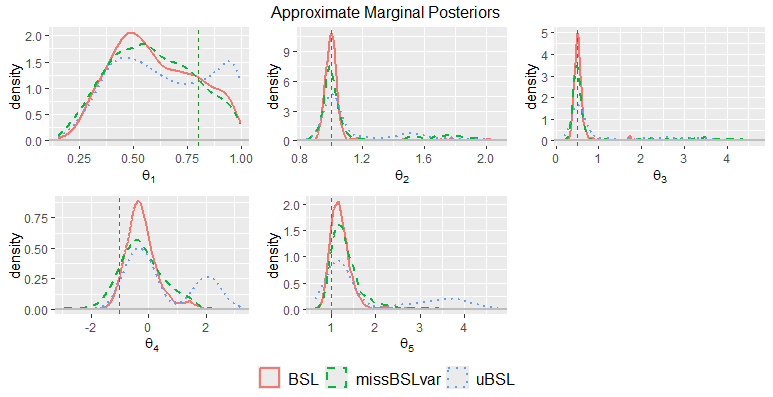
\includegraphics[width=340pt, height=200pt]{Chapters/chapter15/figures/BLSgkSim.png}
	\caption[List of figure caption goes here]{Posterior distributions using Bayesian synthetic likelihood: Simulation exercise g-and-k distribution.}\label{figSBLsimgk}
\end{figure}

\begin{tcolorbox}[enhanced,width=4.67in,center upper,
	fontupper=\large\bfseries,drop shadow southwest,sharp corners]
	\textit{R code. Bayesian synthetic likelihood: Simulation exercise g-and-k distribution.}
	\begin{VF}
		\begin{lstlisting}[language=R]
rm(list = ls()); set.seed(010101)
library(BSL)
# Simulate g-and-k data
RGKnew <- function(par) {
	z <- NULL
	theta <- par[1]; a <- par[2]; b <- par[3]; g <- par[4]; k <- par[5]
	e <- rnorm(n + 1)
	for(t in 2:(n + 1)){
		zt <- e[t] + theta * e[t-1]
		z <- c(z, zt)
	}
	zs <- z / (1 + theta^2)^0.5
	x <- a + b * (1 + 0.8 * (1 - exp(-g * zs)) / (1 + exp(-g * zs))) * (1 + zs^2)^k * zs
	return(x)
}
# Summary statistics
SumSt <- function(y) {
	Oct <- quantile(y, c(0.125, 0.25, 0.375, 0.5, 0.625, 0.75, 0.875))
	eta1 <- Oct[6] - Oct[2]
	eta2 <- (Oct[6] + Oct[2] - 2 * Oct[4]) / eta1
	eta3 <- (Oct[7] - Oct[5] + Oct[3] - Oct[1]) / eta1
	autocor <- acf(y, lag = 2, plot = FALSE)
	autocor[["acf"]][2:3]
	Etay <- c(Oct[4], eta1, eta2, eta3, autocor[["acf"]][2:3])
	return(Etay)
}
# Prior function
LogPrior <- function(par){
	LogPi <- log(par[1] > -1 & par[1] < 1 & par[2] > 0 & par[2] < 5 & par[3] > 0 & par[3] < 5 & par[4] > -5 & par[4] < 5 & par[5] > -0.5 & par[5] < 5)
	return(LogPi)
}
# Population parameters
theta1 <- 0.8; a <- 1; b <- 0.5; g <- -1; k <- 1
parpop <- c(theta1, a, b, g, k)
K <- 5
n <- 500
y <- RGKnew(par = parpop)
# Algorithm parameters
M <- 200 # Number of iterations to calculate mu and sigma
S <- 1100 # Number of MCMC iterations
burnin <- 100 # Burn in iterations
thin <- 2 # Thining parameter
keep <- seq(burnin + 1, S, thin)
par0 <- c(0.5, 2, 1, 0, 1) 
Modelgk <- newModel(fnSim = RGKnew, fnSum = SumSt, theta0 = par0, fnLogPrior = LogPrior, verbose = FALSE)
validObject(Modelgk)
keep <- seq(burnin + 1, S, thin)
tune <- 0.1 # Tuning parameter RW MH
simgk <- simulation(Modelgk, n = M, theta = par0, seed = 10)
par(mfrow = c(2, 3))
\end{lstlisting}
	\end{VF}
\end{tcolorbox}

\begin{tcolorbox}[enhanced,width=4.67in,center upper,
	fontupper=\large\bfseries,drop shadow southwest,sharp corners]
	\textit{R code. Bayesian synthetic likelihood: Simulation exercise g-and-k distribution.}
	\begin{VF}
		\begin{lstlisting}[language=R]
# Check if the summary statistics are roughly normal
for (i in 1:6){
	eval <- seq(min(simgk$ssx[, i]), max(simgk$ssx[, i]), 0.001)
	densnorm <- dnorm(eval, mean = mean(simgk$ssx[, i]), sd(simgk$ssx[, i])) 
	plot(density(simgk$ssx[, i]), main = "", xlab = "")
	lines(eval, densnorm, col = "red")
} 
Lims <- matrix(c(-1, 0, 0, -5, -0.5, 1, rep(5, 4)), 5, 2)
tick <- Sys.time()
Resultsgk <- bsl(y = y, n = M, M = S, model = Modelgk, covRandWalk = tune*diag(5),
method = "BSL", thetaNames = expression(theta, a, b, g, k), 
logitTransformBound = Lims, plotOnTheFly = TRUE)
tock <- Sys.time()
tock - tick
PostChain <- coda::mcmc(Resultsgk@theta[keep,])
CovarRWnew <- var(PostChain)
M <- 500 # Number of iterations to calculate mu and sigma
S <- 6000 # Number of MCMC iterations
burnin <- 1000 # Burn in iterations
thin <- 5 # Thining parameter
keep <- seq(burnin + 1, S, thin)
tune <- 1 # Tuning parameter RW MH
ModelgkNew <- newModel(fnSim = RGKnew, fnSum = SumSt, theta0 = par0, fnLogPrior = LogPrior, verbose = FALSE)
logitTransform <- function(par, a, b){
	logtrans <- log((par - a)/(b - par))
	return(logtrans)
}
ParTrans <- matrix(NA, dim(PostChain)[1], 5)
for(j in 1:5){
	ParTrans[,j] <- logitTransform(par = PostChain[,j], a = Lims[j,1], b = Lims[j,2])
}
CovarRW <- var(ParTrans)
# Vanilla BLS
tick <- Sys.time()
ResultsgkVanila <- bsl(y = y, n = M, M = S, model = ModelgkNew, covRandWalk = tune*CovarRW, method = "BSL", thetaNames = expression(theta, a, b, g, k), logitTransformBound = Lims, plotOnTheFly = TRUE)
tock <- Sys.time()
tock - tick
# Unbiased BLS
tick <- Sys.time()
ResultsgkuBLS <- bsl(y = y, n = M, M = S, model = ModelgkNew, covRandWalk = tune*CovarRW,
method = "uBSL", thetaNames = expression(theta, a, b, g, k),
logitTransformBound = Lims, plotOnTheFly = TRUE)
tock <- Sys.time()
tock - tick
\end{lstlisting}
	\end{VF}
\end{tcolorbox}

\begin{tcolorbox}[enhanced,width=4.67in,center upper,
	fontupper=\large\bfseries,drop shadow southwest,sharp corners]
	\textit{R code. Bayesian synthetic likelihood: Simulation exercise g-and-k distribution.}
	\begin{VF}
		\begin{lstlisting}[language=R]
# Semi-parametric BLS
tick <- Sys.time()
ResultsgksemiBLS <- bsl(y = y, n = M, M = S, model = ModelgkNew, covRandWalk = tune*CovarRW, method = "semiBSL", thetaNames = expression(theta, a, b, g, k),
logitTransformBound = Lims, plotOnTheFly = TRUE)
tock <- Sys.time()
tock - tick
# Misspecified BLS in mean
tick <- Sys.time()
ResultsgkmisspecBLSmean <- bsl(y = y, n = M, M = S, model = ModelgkNew, covRandWalk = tune*CovarRW, method = "BSLmisspec", thetaNames = expression(theta, a, b, g, k),
logitTransformBound = Lims, misspecType = "mean", tau = 0.5, plotOnTheFly = TRUE)
tock <- Sys.time()
tock - tick
# Misspecified BLS in variance
tick <- Sys.time()
ResultsgkmisspecBLSvar <- bsl(y = y, n = M, M = S, model = ModelgkNew, covRandWalk = tune*CovarRW, method = "BSLmisspec", thetaNames = expression(theta, a, b, g, k), 
logitTransformBound = Lims, misspecType = "variance", tau = 0.5, plotOnTheFly = TRUE)
tock <- Sys.time()
tock - tick
# Summary all models
gkResults <- list(ResultsgkVanila, ResultsgkuBLS, ResultsgksemiBLS, ResultsgkmisspecBLSmean, ResultsgkmisspecBLSvar)
names(gkResults) <- c("BSL", "uBSL", "semiBLS", "missBSLmean", "missBSLvar")
t(sapply(gkResults, summary))
combinePlotsBSL(gkResults, which = 2, thetaTrue = parpop, thin = thin, options.linetype = list(values = 1:8), options.size = list(values = rep(1, 8)), options.theme = list(plot.margin = grid::unit(rep(0.03, 4), "npc"), axis.title = ggplot2::element_text(size = 12), axis.text = ggplot2::element_text(size = 8),
legend.text = ggplot2::element_text(size = 12)))
# semi BSL and miss BSL mean are totally diferent to other methods 
gkResultsNew <- list(gkResults[["BSL"]], gkResults[["uBSL"]], gkResults[["missBSLvar"]])
names(gkResultsNew) <- c("BSL", "uBSL", "missBSLvar")
combinePlotsBSL(gkResultsNew, which = 2, thetaTrue = parpop, thin = thin, options.linetype = list(values = 1:8), options.size = list(values = rep(1, 8)), options.theme = list(plot.margin = grid::unit(rep(0.03, 4), "npc"), legend.text = ggplot2::element_text(size = 12)))
\end{lstlisting}
	\end{VF}
\end{tcolorbox}

\item Simulate a multinomial logit model (see Section 6.5 in the book) with 3 alternatives, 2 alternative-specific regressors, and 1 individual-specific regressor. The population parameters for the alternative-specific regressors are $-0.3$ and $1.2$, while the population values for the individual-specific regressor are $0.3$, $0$, and $0.5$. All regressors are assumed to follow a standard normal distribution, and the sample size is 1,000. 

Perform inference using the \textit{INLA} package, and note that the Poisson trick should be used for multinomial models in this exercise (see \cite{serafini2019multinomial} for details).

\textbf{Answer:}

\begin{tcolorbox}[enhanced,width=4.67in,center upper,
	fontupper=\large\bfseries,drop shadow southwest,sharp corners]
	\textit{R code. Multinomial model in INLA: Simulation exercise.}
	\begin{VF}
		\begin{lstlisting}[language=R]
rm(list = ls()); set.seed(010101)
library(INLA)
beta1 <- -0.3; beta2 <- 1.2; gamma <- c(0.3, 0, 0.5)
param <- c(beta1, beta2, gamma); n <- 1000
# Alternative specific regressors
x11 <- rnorm(n); x12 <- rnorm(n); x13 <- rnorm(n)
x21 <- rnorm(n); x22 <- rnorm(n); x23 <- rnorm(n)
# Individual specific regressor
Z <- rnorm(n)
Multinom.sample = function(N){
	Y <- matrix(NA, ncol = 3, nrow = n)
	for(i in 1:n){
		V1 <- beta1*x11[i] + beta2*x21[i] + gamma[1]*Z[i]
		V2<- beta1*x12[i] + beta2*x22[i] + gamma[2]*Z[i]
		V3 <- beta1*x13[i] + beta2*x23[i] + gamma[3]*Z[i]
		probs <- c(V1, V2, V3)
		probs <- exp(probs)/sum(exp(probs))
		samp <- rmultinom(1, N, prob = probs)
		Y[i,] = as.vector(samp)
	}
	colnames(Y ) = c("Y1", "Y2", "Y3")
	return(Y)
}
Y <- Multinom.sample(1)
df <- data.frame(cbind(Y, x11, x12, x13, x21, x22, x23, Z))
Data.structure = function(df){
	Data = matrix(NA, ncol = 6, nrow = n*3)
	for(i in 1:n){
		# simulated variable
		Data[((i-1)*3+1):(i*3), 1] = c(df$Y1[i], df$Y2[i], df$Y3[i])
		# alternative specific with generic coeff
		Data[((i-1)*3+1):(i*3), 2] = c(df$x11[i], df$x12[i], df$x13[i])
		# alternative specific with generic coeff
		Data[((i-1)*3+1):(i*3), 3] = c(df$x21[i], df$x22[i], df$x23[i])
		# individual specific with alternative coeff
		Data[((i-1)*3+1):(i*3), 4] = rep(df$Z[i],3)
		# choice situation index
		Data[((i-1)*3+1):(i*3), 5] = rep(i,3)
		# choice alternative index
		Data[((i-1)*3+1):(i*3), 6] = c(1, 2, 3)
	}
	Data = data.frame(Data)
	names(Data) = c('Y', "X1", "X2", "Z",'phi','alt.idx')
	return(Data)
}
formula = Y ~ -1 + X1 + X2 + f(phi, initial = -10, fixed = T) + f(alt.idx, Z, fixed = T, constr = T)
Data = Data.structure(df)
model = inla(formula, data = Data, family = 'Poisson')
result = rbind(model$summary.fixed[1:5], model$summary.random$alt.idx[2:6])
result = cbind(result, true = param)
\end{lstlisting}
	\end{VF}
\end{tcolorbox}


\begin{tcolorbox}[enhanced,width=4.67in,center upper,
	fontupper=\large\bfseries,drop shadow southwest,sharp corners]
	\textit{R code. Multinomial model in INLA: Simulation exercise.}
	\begin{VF}
		\begin{lstlisting}[language=R]
row.names(result) = c("beta1", "beta2", "gamma.A","gamma.B","gamma.C" )
round(result,3)
diff.result = cbind("0.025quant"= diff(model$summary.random$alt.idx$`0.025quant`), "0.5quant" = diff(model$summary.random$alt.idx$`0.5quant`), "0.975quant" = diff(model$summary.random$alt.idx$`0.975quant`), "true" = diff(gamma))
row.names(diff.result) = c("gamma.B - gamma.A", "gamma.C - gamma.B")
round(diff.result,3)
\end{lstlisting}
	\end{VF}
\end{tcolorbox}
    

\item Get the expression for the ELBO in the linear regression model with conjugate family. 

\textbf{Answer:}

\begin{align*}
	\text{ELBO}(q(\boldsymbol{\beta},\sigma^2))&=\mathbb{E}_{\boldsymbol{\beta},\sigma^2}[\log p(\boldsymbol{y},\boldsymbol{\beta},\sigma^2\mid\boldsymbol{X})]-\mathbb{E}_{\boldsymbol{\beta},\sigma^2}[\log q(\boldsymbol{\beta},\sigma^2)]\\
	&=\mathbb{E}_{\boldsymbol{\beta},\sigma^2}[\log p(\boldsymbol{y}\mid\boldsymbol{\beta},\sigma^2,\boldsymbol{X})+\log \pi(\boldsymbol{\beta}\mid\sigma^2)+\log(\sigma^2)]\\
	&-\mathbb{E}_{\boldsymbol{\beta},\sigma^2}[\log q(\boldsymbol{\beta}) + \log q(\sigma^2)]\\
	&=\mathbb{E}_{\boldsymbol{\beta},\sigma^2}\left[-\frac{N}{2}\log (2\pi)-\frac{N}{2}\log\sigma^2 - \frac{1}{2\sigma^2}(\boldsymbol{y}-\boldsymbol{X}\boldsymbol{\beta})^{\top}(\boldsymbol{y}-\boldsymbol{X}\boldsymbol{\beta})\right.\\
	&\left.-\frac{K}{2}\log(2\pi)-\frac{K}{2}\log(\sigma^2)-\frac{1}{2}\log|\boldsymbol{B}_0|-\frac{1}{2\sigma^2}(\boldsymbol{\beta}-\boldsymbol{\beta}_0)^{\top}\boldsymbol{B}_0^{-1}(\boldsymbol{\beta}-\boldsymbol{\beta}_0)\right.\\
	&-\left.(\alpha_0/2+1)\log\sigma^2-\frac{\delta_0}{2\sigma^2}+\alpha_0/2\log(\delta_0/2)-\log\Gamma(\alpha_0/2)\right]\\
	&-\left\{\mathbb{E}_{\boldsymbol{\beta},\sigma^2}\left[\frac{K}{2}\log\mathbb{E}_{{\sigma^2}}(1/\sigma^2)-\frac{1}{2}\log|\boldsymbol{B}_n|-\frac{1}{2}\mathbb{E}_{{\sigma^2}}(1/\sigma^2)(\boldsymbol{\beta}-\boldsymbol{\beta}_n)^{\top}\boldsymbol{B}_n^{-1}(\boldsymbol{\beta}-\boldsymbol{\beta}_n)\right.\right.\\
	&\left.\left.-\frac{K}{2}\log(2\pi)-(\alpha_n/2+1)\log\sigma^2-\frac{\delta_n}{2\sigma^2}+\alpha_n/2\log(\delta_n/2)-\log\Gamma(\alpha_n/2)\right]\right\}\\
	&=-\frac{N}{2}\log (2\pi)-\frac{1}{2}\log|\boldsymbol{B}_0|+\frac{1}{2}\log|\boldsymbol{B}_n|+\alpha_0/2\log(\delta_0/2)\\
	&-\alpha_n/2\log(\delta_n/2)-\log\Gamma(\alpha_0/2)+\log\Gamma(\alpha_n/2)-\frac{K}{2}\log\mathbb{E}_{{\sigma^2}}(1/\sigma^2)\\
	&+\frac{1}{2}\mathbb{E}_{{\sigma^2}}(1/\sigma^2)\mathbb{E}_{\boldsymbol{\beta}}\left[(\boldsymbol{\beta}-\boldsymbol{\beta}_n)^{\top}\boldsymbol{B}_n^{-1}(\boldsymbol{\beta}-\boldsymbol{\beta}_n)\right]\\
	&=-\frac{N}{2}\log (2\pi)-\frac{1}{2}\log|\boldsymbol{B}_0|+\frac{1}{2}\log|\boldsymbol{B}_n|+\alpha_0/2\log(\delta_0/2)\\
	&-\alpha_n/2\log(\delta_n/2)-\log\Gamma(\alpha_0/2)+\log\Gamma(\alpha_n/2)-\frac{K}{2}\log(\alpha_n/\delta_n)\\
	&+0.5tr\left\{Var(\boldsymbol{\beta})\boldsymbol{B}_n^{-1}\right\}
\end{align*}
We take into account in the fourth equality that the terms collecting $\log\sigma^2$ and $\frac{1}{2\sigma^2}$ cancel out by the definitions of $\alpha_n$ and $\delta_n$, respectively.

\item \textbf{Linear regression continues}

Perform inference in the linear regression example using stochastic variational inference via the automatic differentiation variational inference (ADVI) approach \cite{kucukelbir2017automatic}, implemented in \texttt{rstan} package. In particular, consider the model $y_i = \boldsymbol{x}_i^{\top} \boldsymbol{\beta} + \mu_i$, assuming non-informative independent priors: $\boldsymbol{\beta} \sim N(\boldsymbol{\beta}_0, \boldsymbol{B}_0)$ and $\sigma^2 \sim \mathrm{IG}(\alpha_0/2, \delta_0/2)$, where $\boldsymbol{\beta}_0 = \boldsymbol{0}_3$, $\boldsymbol{B}_0 = 1000\boldsymbol{I}_3$, and $\alpha_0 = \delta_0 = 0.01$. The sample size is one hundred thousand.

\textbf{Answer:}

The posterior mean values are very close to the population parameters, but the 95\% credible intervals are too narrow and do not contain the true values.

\begin{tcolorbox}[enhanced,width=4.67in,center upper,
	fontupper=\large\bfseries,drop shadow southwest,sharp corners]
	\textit{R code. Stochastic variational inference: Simulation exercise linear regression.}
	\begin{VF}
		\begin{lstlisting}[language=R]
library(rstan)
# --- Simulated data ---
N <- 100000; K <- 2; B <- rep(1, K + 1); sig2 <- 1
X <- cbind(1, matrix(rnorm(N * K), N, K))
y <- X %*% B + rnorm(N, 0, sig2^0.5)
# --- Priors ---
b0 <- 0; B0 <- 1000; a0 <- 0.01; d0 <- 0.01
# --- Prepare data for Stan ---
data_list <- list(
N = N,
K = K + 1,  # K+1 because of the intercept
X = X,
y = as.vector(y),
b0 = b0,
B0 = B0,
a0 = a0,
d0 = d0
)
# --- Stan model compilation ---
stan_model_code <- "
data {
	int<lower=0> N;        // number of data points
	int<lower=0> K;        // number of predictors
	matrix[N, K] X;        // predictor matrix
	vector[N] y;           // response vector
	real b0;               // location parameter prior on beta
	real<lower=0> B0;      // variance parameter prior on beta
	real<lower=0> a0;      // shape parameter prior on sigma^2
	real<lower=0> d0;      // rate parameter prior on sigma^2
}
parameters {
	vector[K] beta;        // coefficients of the linear model
	real<lower=0> sigma2;  // variance parameter (sigma^2)
}
model {
	// Priors
	beta ~ normal(b0, B0);       // Normal prior on beta
	sigma2 ~ inv_gamma(a0/2, d0/2); // Inverse Gamma prior
	
	// Likelihood
	y ~ normal(X * beta, sqrt(sigma2)); // Normal likelihood with linear predictor
}
generated quantities {
	vector[N] y_pred;
	for (n in 1:N) {
		y_pred[n] = normal_rng(dot_product(X[n], beta), sqrt(sigma2));
	}
}
"
\end{lstlisting}
	\end{VF}
\end{tcolorbox}

\begin{tcolorbox}[enhanced,width=4.67in,center upper,
	fontupper=\large\bfseries,drop shadow southwest,sharp corners]
	\textit{R code. Stochastic variational inference: Simulation exercise linear regression.}
	\begin{VF}
		\begin{lstlisting}[language=R]
# Compile Stan model
stan_model <- stan_model(model_code = stan_model_code)
# --- Perform Stochastic Variational Inference (SVI) ---
fit <- vb(stan_model, data = data_list, algorithm = "meanfield", iter = 10000)
# --- Extract the results ---
mu_estimate <- extract(fit)$beta
summary(coda::mcmc(mu_estimate))
sigma2_estimate <- extract(fit)$sigma2
summary(coda::mcmc(as.vector(sigma2_estimate)))
		\end{lstlisting}
	\end{VF}
\end{tcolorbox}

\item Let's retake the mixture regression model of Chapter \ref{chap11}, that is, the simple regression mixture with two components such that $z_{i1}\sim \text{Ber}(0.5)$, consequently, $z_{i2}=1-z_{i1}$, and assume one regressor, $x_i\sim N(0,1)$, $i=1,2,\dots,1,000$. Then, 
$$p(y_i \mid \boldsymbol{x}_i) = 
0.5 \phi(y_i \mid 2+1.5x_i,1^2)+0.5 \phi(y_i \mid -1+0.5x_i,0.8^2).$$
Let's set $\alpha_{h0}=\delta_{h0}=0.01$, $\boldsymbol{\beta}_{h0}=\boldsymbol{0}_2$, $\boldsymbol{B}_{h0}=\boldsymbol{I}_2$, and $\boldsymbol{a}_0=[1/2 \ 1/2]^{\top}$.

Perform VB inference in this model using the CAVI algorithm.\\

\textbf{Answer:}

The likelihood function in this model is $p(\bm{y}\mid \bm{z},\bm{\beta},\bm{\sigma}^2)=\prod_{i=1}^N\prod_{h=1}^H\phi(y_i\mid\bm{x}_i^{\top}\bm{\beta}_h,\sigma_h^2)^{z_{ih}}$, and $\pi(\bm{z}\mid\bm{\lambda})=\prod_{i=1}^N\prod_{h=1}^H\lambda_h^{z_{ih}}$, $\bm{\lambda}\sim Dir(\bm{a}_0)$, $\bm{\beta}_h\sim N(\bm{\beta}_{h0},\bm{B}_{h0})$ and $\sigma_h^2\sim IG(\alpha_{h0}/2,\delta_{h0}/2)$. In this notation, $\bm{z},\bm{\beta},\bm{\sigma}^2$ and $\bm{\lambda}$ stacks all the latent indicators, all locations and scale parameters of each cluster, and all the probabilities, respectively. 

Let's work with the mean-field variational family $q(\bm{z},\bm{\lambda},\bm{\beta},\bm{\sigma}^2)=q(\bm{z})q(\bm{\lambda})\prod_{h=1}^H q(\bm{\beta}_h)\prod_{h=1}^H q({\sigma}^2_h)$.

Then,
\begin{align*}
	\log q(\bm{z})=&\mathbb{E}_{\bm{\lambda},\bm{\beta},\bm{\sigma}^2}\left[\log p(\bm{y},\bm{z},\bm{\beta},\bm{\sigma}^2)\right] + c_1\\
	=&\mathbb{E}_{\bm{\lambda},\bm{\beta},\bm{\sigma}^2}\left[\log p(\bm{y}\mid\bm{z},\bm{\beta},\bm{\sigma}^2)+\log \pi(\bm{z}\mid\bm{\lambda})\right] + c_2\\
	=&\mathbb{E}_{\bm{\lambda},\bm{\beta},\bm{\sigma}^2}\left[\sum_{i=1}^N\sum_{h=1}^H z_{ih}\left\{-0.5\log 2\pi - 0.5 \log \sigma^2_h - \right.\right.\\
	&\left.\left.-\frac{1}{2\sigma^2_h}(y_i-\bm{x}_i\bm{\beta}_h)^2 + \log\lambda_h\right\}\right] + c_2\\
	&=\sum_{i=1}^N\sum_{h=1}^H\psi_{ih}\log \rho_{ih} + c_2.
\end{align*}
Thus, $q(\bm{z})=\prod_{i=1}^N\prod_{h=1}^H r_{ih}^{z_{ih}}$, such that $\mathbb{E}_{z_{ih}}[z_{ih}]=r_{ih}$, where $r_{ih}=\frac{\rho_{ih}}{\sum_{j=1}^H\rho_{ij}}$, and
\begin{align*}
	\log \rho_{ih}&=-0.5\log 2\pi -0.5\mathbb{E}_{\sigma^2_h} \log \sigma_h^2 - 0.5 \mathbb{E}_{\sigma^2_h}\left(\frac{1}{\sigma^2_h}\right)\mathbb{E}_{\bm{\beta}_h}(y_i-\bm{x}_i^{\top}\bm{\beta}_h)^2 + \mathbb{E}_{\lambda_h}\log \lambda_h.
\end{align*}
\begin{align*}
	\log q(\bm{\lambda})&=\mathbb{E}_{\bm{z},\bm{\beta},\bm{\sigma}^2}\left[\log p(\bm{y},\bm{z},\bm{\beta},\bm{\sigma}^2)\right]+c_1\\
	&=\mathbb{E}_{\bm{z}}\left[\log \pi(\bm{z}\mid \bm{\lambda})+\log \pi(\bm{\lambda})\right]+c_2\\
	&=\mathbb{E}_{\bm{z}}\left[\sum_{i=1}^N\sum_{h=1}^Hz_{ih}\log \lambda_h+\sum_{h=1}^H(a_{h0}-1)\log \lambda_h\right]+c_3\\
	&=\sum_{i=1}^N\sum_{h=1}^H \mathbb{E}_{z_{ih}}[z_{ih}]\log \lambda_h+\sum_{h=1}^H(a_{h0}-1)\log \lambda_h+c_3\\
	&=\sum_{i=1}^N\sum_{h=1}^H r_{ih}\log \lambda_h+\sum_{h=1}^H(a_{h0}-1)\log \lambda_h+c_3\\
	&=\sum_{h=1}^H \left(\sum_{i=1}^Nr_{ih}+a_{h0}-1\right)\log \lambda_h+c_3.
\end{align*}
This implies that $q(\bm{\lambda})$ is Dirichlet with parameters $a_{hn}=a_{h0}+\sum_{i=1}^N r_{ih}$. 
\begin{align*}
	\log q(\bm{\beta}_h)&=\mathbb{E}_{\bm{\lambda},\bm{z},\bm{\sigma}^2}\left[\log p(\bm{y},\bm{z},\bm{\beta},\bm{\sigma}^2)\right] + c_1\\
	=&\mathbb{E}_{\bm{z},\bm{\sigma}^2}\left[\log p(\bm{y}\mid\bm{z},\bm{\beta},\bm{\sigma}^2)+\log \pi(\bm{\beta}_h)\right] + c_2\\
	&=\mathbb{E}_{\bm{z},\bm{\sigma}^2}\left[\sum_{i=1}^N\sum_{h=1}^Hz_{ih}\left\{-\frac{1}{2\sigma^2_h}(y_i-\bm{x}_i^{\top}\bm{\beta}_h)^2\right\}\right.\\
	&\left. -0.5(\bm{\beta}_h-\bm{\beta}_{h0})^{\top}\bm{B}_{h0}^{-1}(\bm{\beta}_h-\bm{\beta}_{h0})\right]+c_3.
\end{align*}
Following same steps as those to obtain the posterior distribution, and taking into account the expected values, we have that $q(\bm{\beta}_h)$ is $N(\bm{\beta}_{hn},\bm{B}_{hn})$, where $\bm{B}_{hn}=\left(\bm{B}_{h0}^{-1}+\mathbb{E}_{\sigma_h^2}\left(\frac{1}{\sigma^2_h}\right)\sum_{i=1}^Nr_{ih}\bm{x}_i\bm{x}_i^{\top}\right)^{-1}$ and $\bm{\beta}_{hn}=\bm{B}_{hn}\left(\bm{B}_{h0}^{-1}\bm{\beta}_{h0}+\mathbb{E}_{\sigma_h^2}\left(\frac{1}{\sigma^2_h}\right)\sum_{i=1}^Nr_{ih}\bm{x}_iy_i\right)$.
\begin{align*}
	\log q(\sigma_h^2)&=\mathbb{E}_{\bm{\lambda},\bm{z},\bm{\beta}}\left[\log p(\bm{y},\bm{z},\bm{\beta},\bm{\sigma}^2)\right] + c_1\\
	=&\mathbb{E}_{\bm{z},\bm{\beta}}\left[\log p(\bm{y}\mid\bm{z},\bm{\beta},\bm{\sigma}^2)+\log \pi({\sigma}_h^2)\right] + c_2\\
	&=\mathbb{E}_{\bm{z},\bm{\beta}}\left[\sum_{i=1}^N\sum_{h=1}^H z_{ih}\left\{-0.5\log \sigma_h^2-\frac{1}{2\sigma_h^2}(y_i-\bm{x}_i^{\top}\bm{\beta}_h)^2\right\}\right.\\
	&\left.-(\alpha_{h0}/2+1)\log \sigma_h^2-\frac{\delta_{h0}}{2\sigma_h^2}\right]+c_1.
\end{align*}
Collecting terms we see that $q(\sigma_h^2)$ is $IG(\alpha_{hn}/2,\delta_{hn}/2)$, where $\alpha_{hn}=\sum_{i=1}^Nr_{ih}+\alpha_{h0}$ and $\delta_{hn}=\sum_{i=1}^N r_{ih}\mathbb{E}_{\bm{\beta}_h}(y_i-\bm{x}_i^{\top}\bm{\beta}_h)^2+\delta_{h0}$.

Note that the previous results imply that $\mathbb{E}_{\sigma_h^2}\left(\frac{1}{\sigma^2_h}\right)=\alpha_{hn}/\delta_{hn}$, $\mathbb{E}_{\bm{\beta}_h}(y_i-\bm{x}_i^{\top}\bm{\beta}_h)^2=(y_i-\bm{x}_i^{\top}\bm{\beta}_{hn})^2+\bm{x}_i^{\top}\bm{B}_{hn}\bm{x}_i$, and
\begin{align*}
	\log \rho_{ih}&=-0.5\log 2\pi -0.5\mathbb{E}_{\sigma^2_h} \log \sigma_h^2 - 0.5 \mathbb{E}_{\sigma^2_h}\left(\frac{1}{\sigma^2_h}\right)\mathbb{E}_{\bm{\beta}_h}(y_i-\bm{x}_i^{\top}\bm{\beta}_h)^2 + \mathbb{E}_{\lambda_h}\log \lambda_h\\
	&=-0.5\log 2\pi - 0.5(\log(\delta_{hn}/2)-\psi(\alpha_{hn}/2)) - 0.5(\alpha_{hn}/\delta_{hn})(y_i-\bm{x}_i^{\top}\bm{\beta}_{hn})^2\\
	&+\bm{x}_i^{\top}\bm{B}_{hn}\bm{x}_i^{\top} + \psi(a_{hn}) - \psi\left(\sum_{h=1}^Ha_{hn}\right),
\end{align*}
where $\psi$ is the digamma function.

In addition, the evidence lower bound (ELBO) is given by
\begin{align*}
	\text{ELBO}(q(\bm{\theta}))&=\mathbb{E}_q\left[\log p(\bm{y},\bm{z},\bm{\beta},\bm{\sigma}^2)\right]-\mathbb{E}_q[\log q(\bm{z},\bm{\beta},\bm{\sigma}^2)]\\
	&=\mathbb{E}_q\left[\log p(\bm{y}\mid\bm{z},\bm{\beta},\bm{\sigma}^2)+\log\pi(\bm{z}\mid\bm{\lambda})+\log \pi(\bm{\lambda})+\sum_{h=1}^H(\log \pi(\bm{\beta}_h)+\log\pi(\sigma^2_h))\right]\\
	&-\mathbb{E}_q\left[ \log q(\bm{z})+\log \pi(\bm{\lambda})+\sum_{h=1}^H (\log q(\bm{\beta}_h) + \log \pi(\sigma_h^2))\right]\\
	&=\mathbb{E}_q\left[\sum_{i=1}^N\sum_{h=1}^H z_{ih}\left\{-0.5\log (2\pi)-0.5\log\sigma^2_h-0.5\frac{1}{\sigma_h^2}(y_i-\bm{x}_i^{\top}\bm{\beta}_h)^2\right\}\right.\\
	&\left.+\sum_{i=1}^N\sum_{h=1}^Hz_{ih}\log \lambda_h+\sum_{h=1}^H \left\{-\frac{K}{2}\log (2\pi)-0.5\log|\bm{B}_{h0}|-0.5(\bm{\beta}_h-\bm{\beta}_{h0})^{\top}\bm{B}_{h0}^{-1}(\bm{\beta}_h-\bm{\beta}_{h0})\right\}\right.\\
	&\left.+\sum_{h=1}^H\left\{ - (\alpha_{h0}/2+1)\log\sigma_h^2-\frac{\delta_{h0}}{2\sigma_{h}^2}+(\alpha_{h0}/2)\log (\delta_{h0}/2)-\log \Gamma(\alpha_0/2)\right\}\right]\\
	&-\mathbb{E}_q\left[\sum_{i=1}^N\sum_{h=1}^H z_{ih}\log r_{ih}-\log B(\bm{a}_n)+\sum_{h=1}^H(a_{hn}-1)\log \lambda_h\right.\\
	&\left.+\sum_{h=1}^H\left\{-\frac{K}{2}\log (2\pi)-0.5\log|\bm{B}_{hn}|-0.5(\bm{\beta}_h-\bm{\beta}_{hn})^{\top}\bm{B}_{hn}^{-1}(\bm{\beta}_h-\bm{\beta}_{hn})\right\}\right.\\
	&+\left.\sum_{h=1}^H\left\{-(\alpha_{hn}/2+1)\log\sigma_h^2-\frac{\delta_{hn}}{2\sigma_h^2}+(\alpha_{hn}/2)\log (\delta_{hn}/2)-\log \Gamma(\alpha_{hn}/2)\right\}\right].
\end{align*} 
The first part of this expression, that is, $\mathbb{E}_q\left[\log p(\bm{y},\bm{z},\bm{\beta},\bm{\sigma}^2)\right]$, is given by $\sum_{i=1}^N\sum_{h=1}^H r_{ih}\left\{-0.5\log(2\pi)-0.5(\log(\delta_{hn}/2)-\psi(\alpha_{hn}/2)) -\frac{\alpha_{hn}}{2\delta_{hn}}[(y_i-\bm{x}_i^{\top}\bm{\beta}_{hn})^2+\bm{x}_i^{\top}\bm{B}_{hn}\bm{x}_i]\right\}+\sum_{i=1}^N\sum_{h=1}^Hr_{ih}\log r_{it} +\sum_{h=1}^H\left\{-\frac{K}{2}\log (2\pi)-0.5\log|\bm{B}_{h0}|-tr(\bm{B}_{hn}\bm{B}_{h0}^{-1})-(\bm{\beta}_{hn}-\bm{\beta}_{h0})^{\top}(\bm{\beta}_{hn}-\bm{\beta}_{h0})\right\} +\sum_{h=1}^H\left\{-(\alpha_{h0}/2+1)(\log (\delta_{hn}/2)-\psi(\alpha_{hn}/2))-\frac{\delta_{h0}}{2}\frac{\alpha_{hn}}{\delta_{hn}}+(\alpha_{h0}/2)\log(\delta_{h0}/2)-\log\Gamma(\alpha_0/2)\right\}$.

The second part of the ELBO, that is, $\mathbb{E}_q[\log q(\bm{z},\bm{\beta},\bm{\sigma}^2)]$ is given by $\sum_{i=1}^N\sum_{h=1}^Hr_{ih}\log r_{ih}-\log B(\bm{a}_n)+\sum_{h=1}^H(a_{hn}-1)\left(\psi(a_{hn})-\psi\left(\sum_{h=1}^Ha_{hn}\right)\right)+\sum_{h=1}^H-\frac{K}{2}(\log (2\pi)+1)-0.5\log |\bm{B}_{hn}|+(\alpha_{hn}/2+1)\psi(\alpha_{hn}/2)-0.5\alpha_{hn}-\log (\delta_{hn}/2)-\log \Gamma(\alpha_{hn}/2)$. 
We use \begin{align*}
	\mathbb{E}_{\bm{\beta}_h}[(\bm{\beta}_h-\bm{\beta}_{hn})^{\top}\bm{B}_{hn}^{-1}(\bm{\beta}_h-\bm{\beta}_{hn})]&=tr\left\{\mathbb{E}_{\bm{\beta}_h}(\bm{\beta}_h-\bm{\beta}_{hn})^{\top}\bm{B}_{hn}^{-1}(\bm{\beta}_h-\bm{\beta}_{hn})\right\}\\
	&=\mathbb{E}_{\bm{\beta}_h}[tr\left\{(\bm{\beta}_h-\bm{\beta}_{hn})^{\top}\bm{B}_{hn}^{-1}(\bm{\beta}_h-\bm{\beta}_{hn})\right\}]\\
	&=tr\left\{\mathbb{E}_{\bm{\beta}_h}[(\bm{\beta}_h-\bm{\beta}_{hn})(\bm{\beta}_h-\bm{\beta}_{hn})^{\top}\bm{B}_{hn}^{-1}]\right\}\\
	&=tr\left\{Var(\bm{\beta}_h)\bm{B}_{hn}^{-1}\right\}\\
	&=tr\left\{\bm{I}_K\right\}\\
	&=K  
\end{align*}
%The following code implements the CAVI algorithm.
\begin{tcolorbox}[enhanced,width=4.67in,center upper,
	fontupper=\large\bfseries,drop shadow southwest,sharp corners]
	\textit{R code. Variational Bayes: Mixture Gaussian regression.}
	\begin{VF}
		\begin{lstlisting}[language=R]
rm(list = ls())
set.seed(010101)
# Simulate data from a 2-component mixture model
n <- 1000
K <- 2; H <- 2
x <- rnorm(n)
z <- rbinom(n, 1, 0.5)  # Latent class indicator
y <- ifelse(z == 0, rnorm(n, 2 + 1.5*x, 1), rnorm(n, -1 + 0.5*x, 0.8))
X <- cbind(1,x)
# Iterations
S <- 10000
##### From scratch ######
# Hyperparameters
b0h <- rep(0, K); B0h <- diag(1000,K); B0hi <- solve(B0h) 
a0h <- 0.01; d0h <- 0.01; a0 <- rep(1/H, H)
# Innitial values
dhn <- c(50, 50); ahn <- c(500, 500)
bhn <- matrix(c(2, 1.5, -1, 0.5), K, H)
Bhn <- array(c(1,0,0,1,1,0,0,1), c(K, K, H))
an <- c(500, 500)
VarParPsi <- function(dhn, ahn, bhn, Bhn, an){
	logrhoih <- matrix(NA, n, H)
	for(i in 1:n){
		for(h in 1:H){
			logrhoih[i,h] <- -0.5*log(2*pi) - 0.5*(log(dhn[h]/2) - digamma(ahn[h]/2)) -
			0.5*(ahn[h]/dhn[h])*((y[i] - t(X[i,])%*%bhn[,h])^2 + t(X[i,])%*%Bhn[,,h]%*%X[i,]) +
			digamma(an[h]) - digamma(sum(an))
		}
	}
	rhoih <- exp(logrhoih - apply(logrhoih, 1, max)) 
	rih <- rhoih / rowSums(rhoih)
	return(rih)
}
Rih <- VarParPsi(dhn = dhn, ahn = ahn, bhn = bhn, Bhn = Bhn, an = an)
VarParLambda <- function(rih){
	an <- a0 + colSums(rih)
	return(an)
}
VarParLambda(rih = Rih)
VarParBetah <- function(ahn, dhn, rh){
	rXX <- matrix(0, K, K)
	rXy <- matrix(0, K, 1)
	for(i in 1:n){
		rXXi <- rh[i]*X[i,]%*%t(X[i,])
		rXX <- rXX + rXXi
		rXyi <- rh[i]*X[i,]*y[i]
		rXy <- rXy + rXyi
	}
	Bhn <- solve(B0hi + ahn/dhn * rXX)
	bhn <- Bhn%*%(B0hi%*%b0h + ahn/dhn * rXy)
	return(list(bhn = bhn, Bhn = Bhn))
}
\end{lstlisting}
	\end{VF}
\end{tcolorbox}

\begin{tcolorbox}[enhanced,width=4.67in,center upper,
	fontupper=\large\bfseries,drop shadow southwest,sharp corners]
	\textit{R code. Variational Bayes: Mixture Gaussian regression.}
	\begin{VF}
		\begin{lstlisting}[language=R]
VarParSigma2h <- function(bhn, Bhn, rh){
	ahn <- a0h + sum(rh); dhnterm <- 0
	for(i in 1:n){
		dhntermi <- rh[i]*((y[i] - t(X[i,])%*%bhn)^2 + t(X[i,])%*%Bhn%*%X[i,])
		dhnterm <- dhnterm + dhntermi
	}
	dhn <- dhnterm + d0h; return(list(ahn = ahn, dhn = dhn))
}
multivariate_beta <- function(alpha) {
	prod_gammas <- sum(sapply(alpha, lgamma))
	sum_alpha <- sum(alpha)
	gamma_sum_alpha <- lgamma(sum_alpha)
	return(prod_gammas - gamma_sum_alpha)
}
ELBO <- function(rih, dhn, ahn, bhn, Bhn, an){
	LogLikh <- 0; LogPrioPsih <- 0
	LogPriorBeta <- 0; LogPriorSig2 <- 0
	for(h in 1:H){
		for(i in 1:n){
			LogLikih <- rih[i, h]*(-0.5*log(2*pi) - 0.5*(log(dhn[h]/2) - digamma(ahn[h]/2)) - 0.5*(ahn[h]/dhn[h])*((y[i] - t(X[i,])%*%bhn[,h])^2 + t(X[i,])%*%Bhn[,,h]%*%X[i,]))
			LogLikh <- LogLikh + LogLikih
			LogPrioPsiih <- rih[i, h]*(digamma(an[h]) - digamma(sum(an)))
			LogPrioPsih <- LogPrioPsih + LogPrioPsiih
		}
		LogPriorBetah <- -0.5*K*log(2*pi) - 0.5*log(det(B0h)) - sum(diag(Bhn[,,h]%*%B0hi)) - t(bhn[,h] - b0h)%*%B0hi%*%(bhn[,h] - b0h)
		LogPriorBeta <- LogPriorBeta + LogPriorBetah
		LogPriorSig2h <- -(a0h/2+1)*(log(dhn[h]/2) - digamma(ahn[h]/2)) - 0.5*d0h*(ahn[h]/dhn[h]) + (a0h/2)*log(d0h/2) - lgamma(a0h/2)
		LogPriorSig2 <- LogPriorSig2 + LogPriorSig2h  
	}
	LogJoint <- LogLikh + LogPrioPsih + LogPriorBeta + LogPriorSig2
	logqPsi <- 0; logqLambda <- 0; logqBeta <- 0;logqSig2 <- 0
	for(h in 1:H){
		for(i in 1:n){
			logqPsiih <- rih[i, h] * log(rih[i, h])
			logqPsi <- logqPsi + logqPsiih
		}
		logqLambdah <- (an[h] - 1)*(digamma(an[h]) - digamma(sum(an)))
		logqLambda <- logqLambda + logqLambdah
		logqBetah <- -0.5*K*log(2*pi + 1) - 0.5*log(det(Bhn[,,h])) 
		logqBeta <- logqBeta + logqBetah
		logqSig2h <- -log(dhn[h]/2) + (ahn[h]/2+1)*digamma(ahn[h]/2) - ahn[h]/2 - lgamma(ahn[h]/2)
		logqSig2 <- logqSig2 + logqSig2h
	}
	logqLambda <- logqLambda - multivariate_beta(alpha = an)
	logq <- logqPsi + logqLambda + logqBeta + logqSig2
	ELBO <- LogJoint - logq
	return(ELBO)
}
\end{lstlisting}
	\end{VF}
\end{tcolorbox}

\begin{tcolorbox}[enhanced,width=4.67in,center upper,
	fontupper=\large\bfseries,drop shadow southwest,sharp corners]
	\textit{R code. Variational Bayes: Mixture Gaussian regression.}
	\begin{VF}
		\begin{lstlisting}[language=R]
# Initial values
fit_lm1 <- lm(y ~ x)
bhn[,1] <- coef(fit_lm1)
bhn[,2] <- coef(fit_lm1) + rnorm(K, 0, 0.5) 
Bhn[,,1] <- diag(0.1, K); Bhn[,,2] <- diag(0.1, K)
ahn <- rep(10, H); dhn <- rep(10, H)
an <- c(300, 700)
ELBOs <- rep(NA, S)
ELBOs[1] <- ELBO(rih = Rih, dhn = dhn, ahn = ahn, bhn = bhn, Bhn = Bhn, an = an)
epsilon <- 1e-5
for(s in 2:S){
	Rih <- VarParPsi(dhn = dhn, ahn = ahn, bhn = bhn, Bhn = Bhn, an = an)
	an <- VarParLambda(rih = Rih)
	bhn <- matrix(NA, K, H)
	Bhn <- array(NA, c(K, K, H))
	for(h in 1:H){
		EnsVarParBetah <- VarParBetah(ahn = ahn[h], dhn = dhn[h], rh = Rih[,h])
		bhn[,h] <- EnsVarParBetah[["bhn"]]
		Bhn[,,h] <- EnsVarParBetah[["Bhn"]] 
	}
	ahn <- rep(NA, H)
	dhn <- rep(NA, H)
	for(h in 1:H){
		EnsVarParSig2h <- VarParSigma2h(bhn = bhn[,h], Bhn = Bhn[,,h], rh = Rih[,h])
		ahn[h] <- EnsVarParSig2h[["ahn"]]
		dhn[h] <- EnsVarParSig2h[["dhn"]] 
	}
	ELBOs[s] <- ELBO(rih = Rih, dhn = dhn, ahn = ahn, bhn = bhn, Bhn = Bhn, an = an)
	# Check if lower bound decreases
	if (ELBOs[s] < ELBOs[s - 1]) { message("Lower bound decreases!\n")}
	# Check for convergence
	if (ELBOs[s] - ELBOs[s - 1] < epsilon) { break }
	# Check if VB converged in the given maximum iterations
	if (s == S) {warning("VB did not converge!\n")}
}
plot(ELBOs[1:s], type = "l", main = "ELBO over iterations", ylab = "ELBO", xlab = "Iteration")
Sig21 <- MCMCpack::rinvgamma(S, ahn[1]/2, dhn[1]/2) 
summary(coda::mcmc(Sig21))
Sig22 <- MCMCpack::rinvgamma(S, ahn[2]/2, dhn[2]/2) 
summary(coda::mcmc(Sig22))
Beta1 <- MASS::mvrnorm(S, mu = bhn[,1], Sigma = Bhn[,,1])
summary(coda::mcmc(Beta1))
Beta2 <- MASS::mvrnorm(S, mu = bhn[,2], Sigma = Bhn[,,2])
summary(coda::mcmc(Beta2))
Lambda <- MCMCpack::rdirichlet(S, alpha = an)
summary(coda::mcmc(Lambda))
\end{lstlisting}
	\end{VF}
\end{tcolorbox}

\end{enumerate}